\begin{table}[htbp]
\centering\small
\caption{Change in balanced H0 fixed-bin yield versus an equal-update no-new-data continuation, in percentage points, mean $\pm$ sample SD over three paired fit/proposal seeds. Round 2 uses the same first-round lineage as its control. The rounds have separate assessment histories.}
\begin{tabular}{lrrrr}\toprule
Model / rule & UMA r1 & UMA r2 & MACE r1 & MACE r2\\\midrule
AR / fixed & $-1.33\pm1.61$ & $+1.39\pm0.53$ & $-1.50\pm0.85$ & $+1.27\pm0.35$\\
AR / adaptive & $-0.35\pm1.51$ & $+0.61\pm0.60$ & $+0.03\pm2.23$ & $+0.14\pm0.90$\\
AR / range & $+6.57\pm2.36$ & $-5.41\pm1.48$ & $+6.13\pm1.35$ & $-6.31\pm1.65$\\
CVAE $D=2$ / fixed & $-0.90\pm0.88$ & $-0.17\pm0.68$ & $-0.69\pm1.00$ & $-0.55\pm0.56$\\
CVAE $D=2$ / adaptive & $+0.17\pm1.61$ & $+0.43\pm0.63$ & $+0.12\pm1.66$ & $+0.26\pm0.77$\\
CVAE $D=2$ / range & $+6.08\pm1.97$ & $-6.28\pm1.76$ & $+6.16\pm1.25$ & $-6.22\pm1.48$\\
\bottomrule\end{tabular}
\end{table}


Range labels improve the first-round balanced statistic by about six points
under both teachers, but the second acquired batch reverses that gain
relative to the appropriate continuation. The first-round same-data
range-minus-fixed contrast is $+7.90\pm0.83$ points for AR and
$+6.97\pm2.74$ for $D=2$ under UMA. Most of that gain is HIGH-class
conditioning: AR's fixed-LOW change is only $+0.35$ points, whereas its
HIGH change is $+29.77$ points. A broad-class gain is not an equally large
gain in low-energy discovery.

\begin{figure}[htbp]
\centering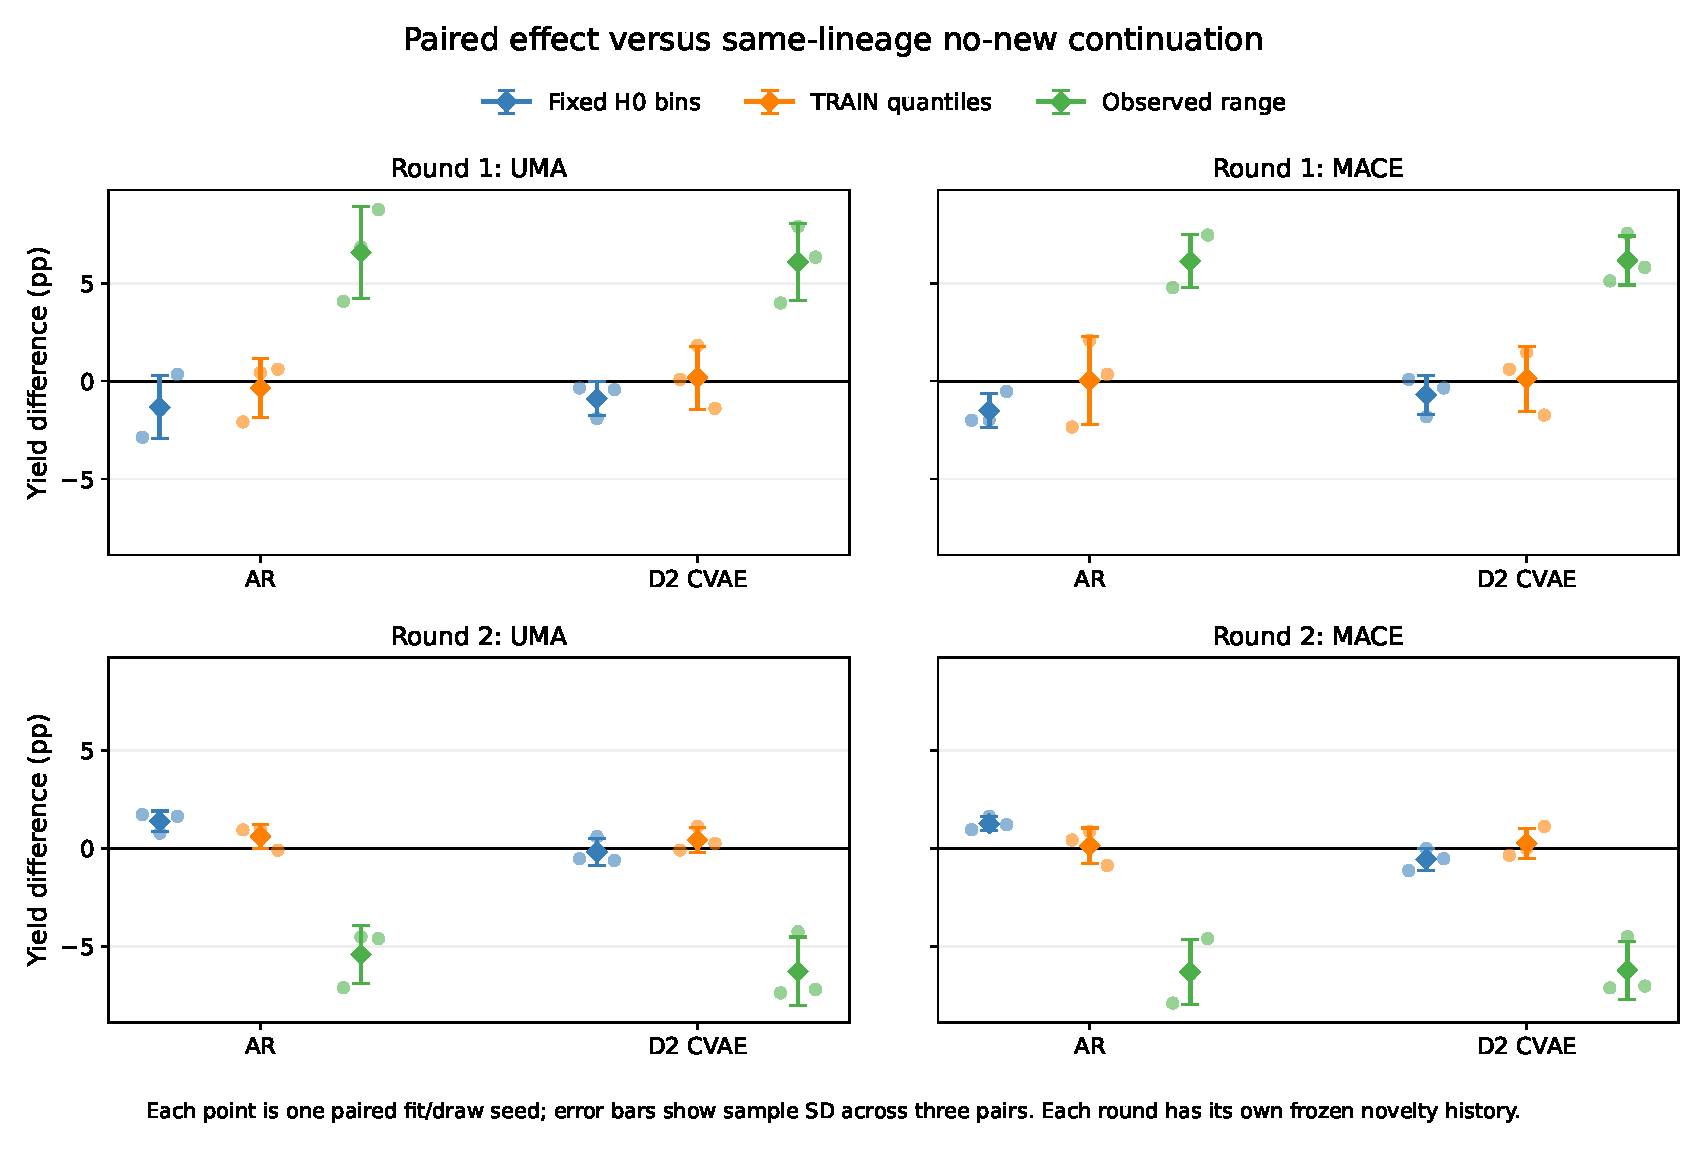
\includegraphics[width=\linewidth]{iteration_paired_gains.pdf}
\caption{Acquisition effects within separately frozen assessments. Each
round uses its appropriate no-new-data continuation; round 2 starts both
arms from the same first-round lineage. Error bars are SD over three paired
fit/proposal seeds.}
\end{figure}

After round two, absolute UMA range yields remain 70.28\% for AR and
68.66\% for $D=2$, above the declared fresh uniform and fixed-TRAIN-seed
mutation baselines of $33.88\pm0.59$\% and $58.16\pm1.53$\%. Nevertheless,
continuing the first-round model without the new range batch performs better.
The decline mainly appears in fixed-bin condition fidelity; novelty still
exceeds 97\%.

This requires care in interpretation. Acquiring higher-energy extrema raises
the range-defined LOW cutoff, so the requested target itself becomes less
strict relative to the fixed-H0 LOW reference. The negative fixed-metric
change and the positive extension of upper-energy coverage describe different
outcomes. The detailed report separates novelty, condition fidelity, moving
bins, endpoint growth, and loss-weight concentration rather than reducing
them to one success label.

\begin{table}[htbp]
\centering\small
\caption{Posthoc conditioning/data controls: balanced H0 fixed-bin yield change, percentage points, mean $\pm$ sample SD over three paired fits. Relabeling also changes class-balanced loss weights. The matched-range comparison holds the physical edges identical; adding rows can still change minibatches and row weights.}
\begin{tabular}{lrr}\toprule
Model / contrast & UMA & MACE\\\midrule
AR / H0 range versus fixed & $+6.48\pm1.01$ & $+6.11\pm0.98$\\
AR / New rows / fixed edges & $-1.56\pm0.88$ & $-1.10\pm1.33$\\
AR / New rows / matched range edges & $-1.36\pm0.39$ & $-2.05\pm0.84$\\
CVAE $D=2$ / H0 range versus fixed & $+7.06\pm1.09$ & $+6.80\pm0.91$\\
CVAE $D=2$ / New rows / fixed edges & $+0.41\pm0.78$ & $+0.09\pm0.46$\\
CVAE $D=2$ / New rows / matched range edges & $+1.85\pm1.33$ & $+2.00\pm1.39$\\
\bottomrule\end{tabular}
\end{table}


A fresh, explicitly post-hoc control shows that most of the first-round
range-label gain does not require new structures. Starting from the same
original checkpoint and allocating the same 2,000-update continuation,
relabeling H0 alone improves balanced UMA yield by $6.48\pm1.01$ points for
AR and $7.06\pm1.09$ for $D=2$. Independent MACE assessment gives
$6.11\pm0.98$ and $6.80\pm0.91$ points. At identical first-round range edges,
adding the acquired rows instead changes UMA yield by $-1.36\pm0.39$ points
for AR and $+1.85\pm1.33$ for $D=2$; MACE gives $-2.05\pm0.84$ and
$+2.00\pm1.39$ points. These are three-pair sample SDs.

The larger improvement is therefore available through conditioning and its
associated loss reweighting on existing data. The smaller added-row effect
depends on architecture. This does not negate the measured expansion of
upper-energy samples: fixed-bin fidelity and exploration of a wider observed
energy range answer different questions. Neither outcome establishes DFT
accuracy, physical stability, or global coverage.

